\documentclass[10pt,a4paper]{article}
\usepackage[utf8]{inputenc}
\usepackage[spanish]{babel}
\usepackage{amsmath}
\usepackage{amsfonts}
\usepackage{amssymb}
\usepackage{graphicx}
\usepackage{multicol}
\usepackage{titling}
\usepackage{titlesec}
\usepackage{array}
\usepackage{bm}
\usepackage{afterpage}
\usepackage{float}
\usepackage{graphicx}
\usepackage{epstopdf}
\usepackage{longtable}
\usepackage{xcolor}
\usepackage{epigraph}
\setlength\epigraphwidth{1.5\textwidth}
\usepackage{subfigure}
\usepackage{anyfontsize}
\usepackage[left=2cm,right=2cm,top=2cm,bottom=2cm]{geometry}
\usepackage[colorlinks=true,
            linkcolor=blue,
            citecolor=blue,
            urlcolor=blue]{hyperref}

\begin{document}
\author{Lisseth C. Alban-Checa}
\title{SISTEMAS EMBEBIDOS \\
LABORATORIO #1}
\maketitle

\section{Introducción}
\begin{multicols}{2}
Las entradas digitales nos permiten distinguir entre dos estados: activo(encendido)– inactivo(apagado). Arduino UNO(ATmega328p) consta de 14 puertos digitales que pueden funcionar como salidas y como entradas. 
\\-B (pines digitales del 8 al 13)
\\-C (entradas analógicas)
\\-D (pines digitales del 0 al 7)
Cuando actúan como entradas trabajan con dos estados de tensiones: 0V (estado de no activación) y 5V (estado de activación).
\\La comunicación serial entre dos dispositivos se realiza a través del intercambio de una secuencia de bits, donde se transmite bit a bit, uno por vez, donde, aunque es lenta la comunicación, tiene la ventaja de poder ser transmitida a mayores distancias y utilizar menos líneas de comunicación.
La comunicación serial entre dos dispositivos únicamente utiliza 3 líneas las cuales son:
\\-Línea de recepción de datos (RX)
\\-Línea de transmisión de datos (TX)
\\-Línea común (GND)
\end{multicols}

\section{Consulta}
\begin{itemize}
\item Consultar sobre la rotacion de datos dentro de la librerıa LiquidCrystal para realizar la rotacion de palabras ingresadas por teclado matricial.
\\Para la programacion en Arduino vamos a utilizar una librería que nos hará más fácil el desarrollo. Esta librería es LiquidCrystal.h. No hace falta instalarla en el entorno de desarrollo oficial ya que viene por defecto. Lo único que tenemos que hacer es añadirla como un include en nuestro programa o sketch. 
\end{itemize}
\begin{itemize}
\item Presentar el funcionamiento mediante diagrama de bloques y flujo.
\begin{figure}[hb]
\centering
\caption{DIAGRAMA DE FLUJO}
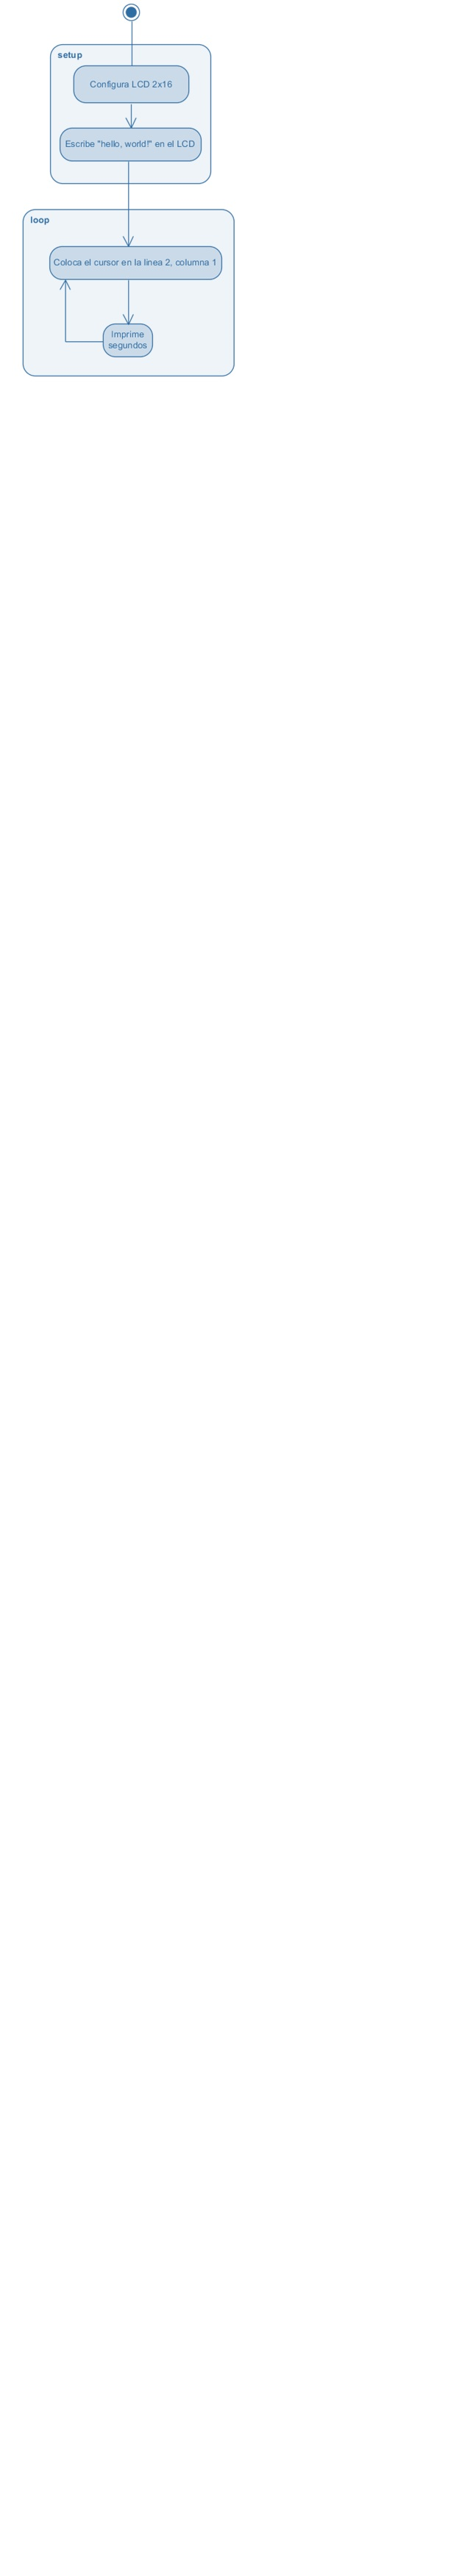
\includegraphics[scale=0.5]{DIAGRAMA DE FLUJO.png}
\end{figure}
\end{itemize}

\section{Ejercicio Propuesto}
\begin{itemize}
\item Se debe dise˜nar un sistema de control de acceso por medio de una contrase˜na individual.
\end{itemize}
\begin{itemize}
\item Las contrase˜nas ya se cuentran establecidas para cada persona y estan almacenadas en el sistema.Estas son: Carlos Arias cod:ca900813, Andres Juarez cod:aj881112 y Javier Andrada cod:ja890109. Estos son ingresados por comunicacion serial.
\end{itemize}
\begin{itemize}
\item Cada usuario debe ingresar su c´odigo y en una LCD deber´a aparecer por rotaci´on de datos: ”BIENVENIDO NOMBRE APELLIDO”.
\end{itemize}
\begin{itemize}
\item Al presionar un boton, se debera presentar como reporte por mensaje serial quien ya ingreso a la empresa y quien no lo ha hecho.
\end{itemize}
\begin{itemize}
\item El resto de restricciones son propuestas por cada estudiante.
\end{itemize}

\section{Desarrollo}
\subsection{Simulación}
\begin{figure}[hb]
\centering
\caption{CODIGO ARDUINO}
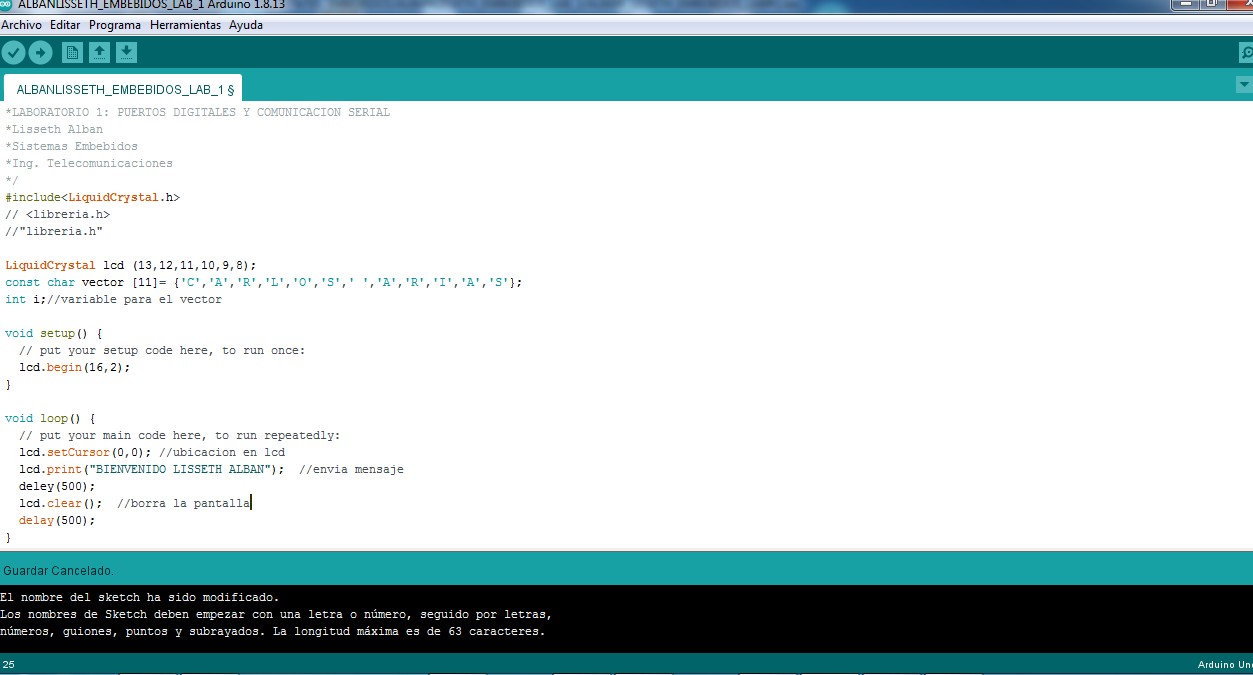
\includegraphics[scale=0.5]{CODIGO ARDUINO.png}
\end{figure}
\begin{figure}[hb]
\centering
\caption{SIMULACION}
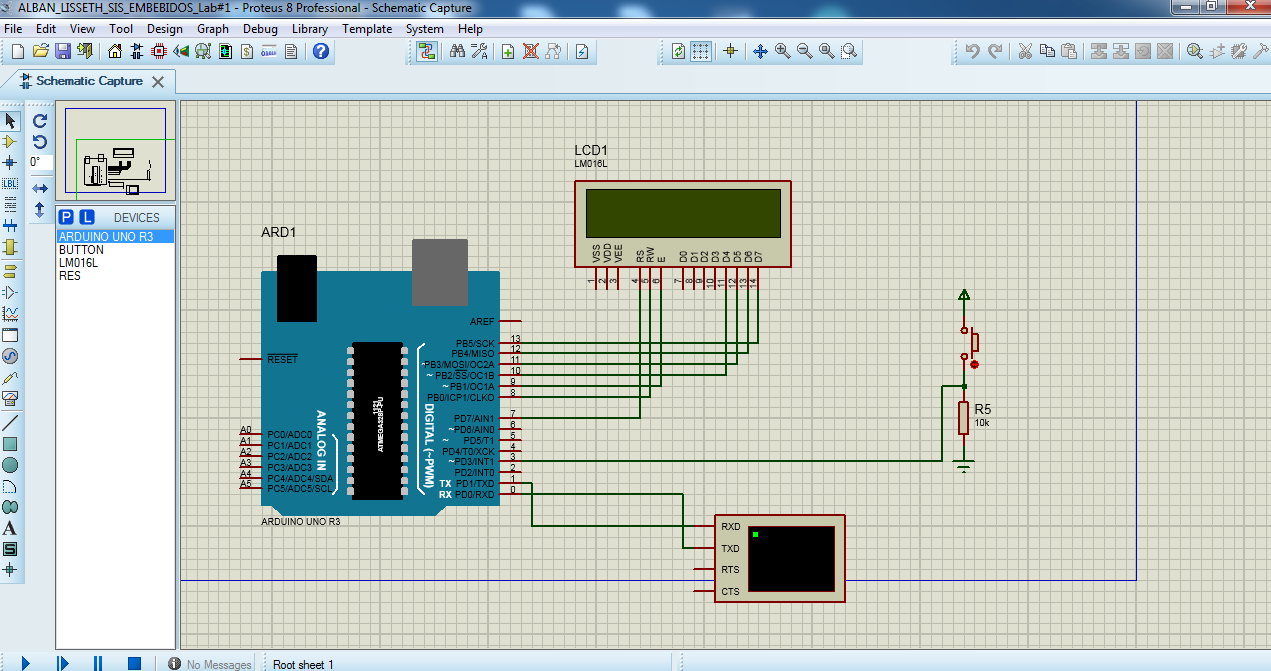
\includegraphics[scale=0.5]{SIMULACION.png}
\end{figure}

\section{Análisis de Resultados}
\begin{itemize}
Como podemos observar el resultado final ha sido satisfactorio ya que podemos observar lo que se nos fue pedido en el desarrollo de este laboratorio con sus respectivos ítems.
\end{itemize}

\section{Conclusiones y Recomendaciones}
\subsection{Conclusiones}
\begin{itemize}
\item La utilizacion de la comunicacion serial es muy util en cuanto al ingreso de claves e informacion que se desea adquirir de manera facil.
\item la utilizacion ddel sistema arduino y la silumacion del program,a proteus es de gran ayuda para el desarrollo de esta materia.
\end{itemize}
\\
\subsection{Recomenciones}
\begin{itemize}
\item revisar que las librerias sean la indicadas para la realizacion de los proyectos a ejecutarse.
\item Saber representar la lógica de programación al sistema de simulación esto hará́ que se facilite los procesos al momento de crear nuestro proyecto.
\end{itemize}

\end{document}